\chapter{Аналитический раздел}
\section{Поверхностное натяжение}
Пузырь существует потому, что поверхность любой жидкости имеет некоторое поверхностное натяжение, которое делает поведение поверхности похожим на поведение чего-нибудь эластичного.

Поверхностное натяжение \cite{surface_tension} — это явление, при котором вещество (прежде всего, жидкость) стремится приобрести форму с минимально возможной площадью поверхности. Это достигается за счет наличия сил поверхностного натяжения.

Сферическая форма пузыря также получается за счёт поверхностного натяжения. Силы натяжения формируют сферу потому, что сфера имеет наименьшую площадь поверхности при данном объёме.  

Важно также упомянуть о мембране между пузырями. Это пленка, разделяющая два пузыря. При образовании кластера она принимает форму сферической поверхности, так как её кривизна уравновешивает разницу давлений. В техническом задании сказано, принять мембрану за плоскость.

\section{Условия образования кластера, отталкивания и слияния}

Основные силы и условия, влияющие на формирование сложных пузырей:
\begin{enumerate}[label={\arabic*)}]
	\item Силы поверхностного натяжения
	\begin{itemize}	
		\item Поверхностное натяжение является ключевым фактором, определяющим форму и стабильность пузырей. Оно стремится минимизировать площадь поверхности пузыря, что приводит к образованию сферических форм.
		\item При взаимодействии нескольких пузырей, силы поверхностного натяжения могут вызывать как слияние, так и отталкивание пузырей.
	\end{itemize}
	\item Избыточное давление
	\begin{itemize}	
		\item Избыточное давление внутри пузыря определяется его радиусом. По формуле Лапласа~\cite{laplace}: \[ \Delta P = \frac{2\sigma}{R} \]
		\item Разница в избыточном давлении между пузырями может приводить к их слиянию или отталкиванию, в зависимости от их размеров и расстояний между ними.
	\end{itemize}
	\item Силы взаимодействия между пузырьками
	\begin{itemize}	
		\item Силы взаимодействия между пузырями, такие как силы Ван дер Ваальса, могут способствовать образованию кластеров. При близком расположении пузырей, силы притяжения могут преобладать над силами отталкивания, что приводит к слиянию.
	\end{itemize}
	\item Вязкость окружающей среды
	\begin{itemize}	
		\item Вязкость воздуха (или жидкости, если пузырьки образуются в жидкости) влияет на динамику движения пузырей. Более вязкие среды замедляют движение пузырей и могут способствовать образованию более стабильных структур.
	\end{itemize}
	\item Температура
	\begin{itemize}	
		\item Температура влияет на свойства жидкости и газов, а также на поверхностное натяжение. При повышении температуры поверхностное натяжение может уменьшаться, что может способствовать образованию пузырей.
	\end{itemize}
	\item Концентрация поверхностно-активных веществ (ПАВ)
	\begin{itemize}	
		\item ПАВ снижают поверхностное натяжение и могут стабилизировать пузырьки, предотвращая их слияние. Они также могут влиять на размер и форму пузырей.
	\end{itemize}
	\item Геометрия и размеры пузырей
	\begin{itemize}	
		\item Размеры и форма пузырей влияют на их взаимодействие. Меньшие пузырьки могут сливаться с большими, что приводит к образованию более крупных пузырей.
	\end{itemize}	
	\item Скорость потока воздуха
	\begin{itemize}	
		\item В условиях течения воздуха пузырьки могут быть вытянуты или деформированы, что влияет на их стабильность и возможность слияния. Высокая скорость потока может привести к образованию более мелких пузырей.
	\end{itemize}	
\end{enumerate}

\section{Геометрическое построение сложных пузырей}

В книге \guillemotleft Мыльные пузыри\guillemotright~\cite{boys} Бойс Ч.В., опираясь на книгу Жозефа Плато \guillemotleft Статика жидкости\guillemotright, описал геометрическое построение, позволяющее точно вычертить два пузыря и разделяющую их перегородку.

\begin{figure}[h]
	\centering
	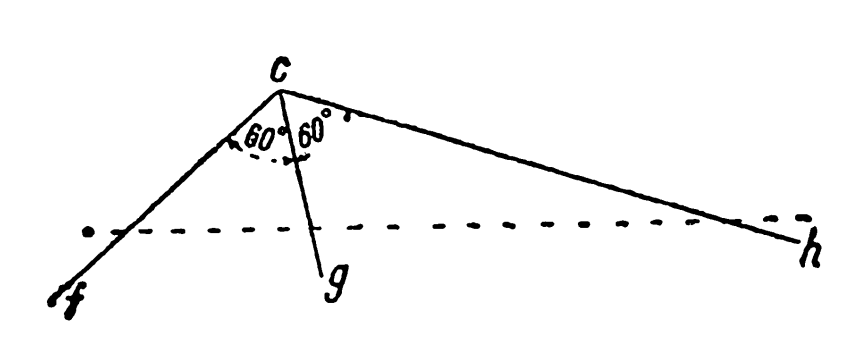
\includegraphics[width=0.5\linewidth]{pictures/drawing_cluster_1.png}
	\caption{Сложные пузыри. Часть 1}
	\label{fig:drawing_cluster_1}
\end{figure}
\begin{figure}[h]
	\centering
	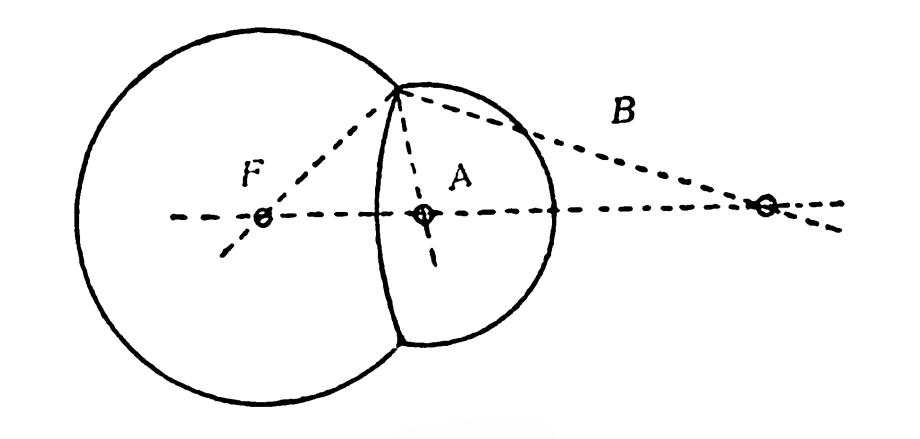
\includegraphics[width=0.7\linewidth]{pictures/drawing_cluster_2.png}
	\caption{Сложные пузыри. Часть 2}
	\label{fig:drawing_cluster_2}
\end{figure}

Из какой-либо точки С проведены три линии: 
Сf, Сg, Сh, образующие два угла по 60°, как показано 
на рис.~\ref{fig:drawing_cluster_1}. Они пересекаются четвертой прямой линией, проведенной на рисунке пунктиром. Получившиеся три точки пересечения являются центрами трех окружностей, соответствующих трем возможным пузырям. 
Точка пересечения средней линии является центром 
окружности малого пузыря, из других же двух точек 
та, которая ближе к С, представляет собой центр второго пузыря, а та, которая находится дальше от С, — центр перегородки. Теперь, устанавливая одну из ножек циркуля последовательно в каждой из этих точек, проведены отрезки окружностей, проходящих через С, как показано на рис.~\ref{fig:drawing_cluster_2}, на котором линии рисунка~\ref{fig:drawing_cluster_1} воспроизведены пунктиром, дуги же окружностей — сплошными линиями~\cite{boys}.

Такое же рассуждение может быть расширено до трёхмерного построения.

\section{Модель взаимодействия двух пузырей при соприкосновении}
\label{sec:model_of_contact}
Поскольку на данный процесс влияет такое большое количество разных факторов и нет единой системы уравнений для определения того, что именно произойдёт с двумя соприкоснувшимися пузырями, и техническое задание требует визуализации, а не моделирования, была введена модель для упрощённого определения взаимодействия двух пузырей. Так как в книге \guillemotleft Мыльные пузыри\guillemotright~\cite{boys} Бойса Ч.В. пузырьковый кластер строится при угле соприкосновения равном шестидесяти градусам, примем следующую модель взаимодействия:
\begin{itemize}	
	\item образование кластера при $55\degree \leq \phi \leq 65\degree$;
	\item образование одного большого пузыря при $\phi < 55\degree$;
	\item отталкивание при $ 65\degree < \phi$;
\end{itemize}
где: $\phi$ --- угол соприкосновения пузырей т.е. наименьший угол между радиусами сфер в любой точке соприкосновения.
	
\section{Обзор существующих методов визуализации трёхмерной сцены}
Проведён обзор следующих методов визуализации трёхмерных сцен:
\begin{enumerate}[label={\arabic*)}]
	\item алгоритм определения видимых поверхностей путём трассировки лучей;
	\item алгоритм, использующий Z-буфер;
	\item алгоритм плавающего горизонта.
\end{enumerate}

\subsection{Алгоритм определения видимых поверхностей путём трассировки лучей}
Главная идея, лежащая в основе этого метода, заключается в том, что наблюдатель видит любой объект посредством испускаемого неким источником света, который падает на этот объект и затем каким-то путем доходит до наблюдателя. Свет может достичь наблюдателя, отразившись от поверхности, преломившись или пройдя через нее. Если проследить за лучами света, выпущенными источником, то можно убедиться, что весьма немногие из них дойдут до наблюдателя. Следовательно, этот процесс был бы вычислительно неэффективен. Поэтому было предложено отслеживать (трассировать) лучи в обратном направлении, т. е. от наблюдателя к объекту, как показано на рис.~\ref{fig:ray_tracing_pic}.
\begin{figure}[h]
	\centering
	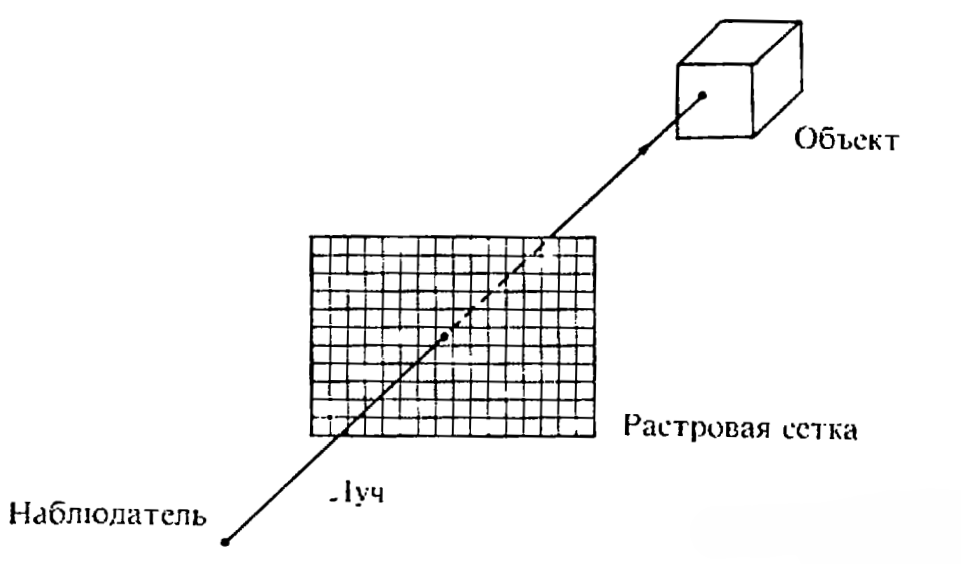
\includegraphics[width=0.6\linewidth]{pictures/ray_tracing_pic.png}
	\caption{Простая трассировка луча}
	\label{fig:ray_tracing_pic}
\end{figure}

Эти алгоритмы учитывают эффекты отражения одного объекта от поверхности другого, преломления, прозрачности и затенения. Производится также устранение ступенчатости.

\textbf{Преимущества:}
\begin{itemize}
	\item учитывает эффект отражения одного объекта от поверхности другого;
	\item учитывает эффект преломления;
	\item учитывает эффект прозрачности;
	\item учитывает эффект затенения;
	\item производит устранение ступенчатости;
	\item позволяет создавать изображения с высокой степенью реалистичности.
\end{itemize}

\textbf{Недостатки:}
\begin{itemize}
	\item требует значительных вычислительных ресурсов;
	\item реализация может быть сложной для динамических сцен.
\end{itemize} 
\subsection{Алгоритм, использующий Z-буффер}
Этот алгоритм работает в пространстве изображения. Идея z-буфера является обобщением идеи о буфере кадра. Буфер кадра используется для запоминания атрибутов (интенсивности) каждого пиксела в пространстве изображения. 

Z-буфер это отдельный буфер глубины, используемый для запоминания координаты z или глубины каждого видимого пиксела в пространстве изображения. В процессе работы глубина или значение z каждого нового пиксела, который нужно занести в буфер кадра, сравнивается с глубиной того пиксела, который уже занесен в z-буфер. Если это сравнение показывает, что новый пиксел расположен впереди пиксела, находящегося в буфере кадра, то новый пиксел заносится в этот буфер и, кроме того, производится корректировка z-буфера новым значением z. Если же сравнение дает противоположный результат, то ни каких действий не производится. По сути, алгоритм является поиском по х и у наибольшего значения функции z (х, у).

\textbf{Преимущества:}
\begin{itemize}
	\item простота\cite{rogers};
	\item решает задачу об удалении невидимых поверхностей;
	\item делает тривиальной визуализацию пересечений сложных поверхностей;
	\item оценка вычислительной трудоемкости алгоритма не более чем линейна и зависит от габаритов пространства изображения.
\end{itemize}

\textbf{Недостатки:}
\begin{itemize}
	\item большой объем требуемой памяти.
\end{itemize}
\subsection{Алгоритм плавающего горизонта}
Алгоритм плавающего горизонта чаще всего используется для удаления невидимых линий трехмерного представления функций, описывающих поверхность в виде:
\[
F(x, y, z) = 0
\]

Главная идея данного метода заключается в сведении трехмерной задачи к двумерной путем пересечения исходной поверхности последовательностью параллельных секущих плоскостей, имеющих постоянные значения координат х, у или z. Для хранения максимальных и минимальных значений у при каждом значении х используются два массива чисел: массив верхнего горизонта и массив нижнего горизонта.

\textbf{Преимущества:}
\begin{itemize}
	\item простота;
	\item метод плавающего горизонта может обрабатывать большие объемы данных в реальном времени.
\end{itemize}

\textbf{Недостатки:}
\begin{itemize}
	\item метод плавающего горизонта может не подходить для визуализации данных, которые требуют высокой степени детализации или точности;
	\item не подходит для реалистичной визуализации с тенями и бликами.
\end{itemize}

\section{Обоснование выбора метода визуализации}
Для реализации был использован алгоритм определения видимых поверхностей путём трассировки лучей. Это было сделано по следующим причинам:
\begin{itemize}
	\item из всех проанализированных ранее алгоритмов с помощью данного можно создать наиболее реалистичное изображение;
	\item можно визуализировать блики;
	\item можно визуализировать отражение объектов друг в друге.
\end{itemize}
\clearpage
